\section{The Landscape of Rationality for Relations over Finite Words}
\label{sec:preliminaries-automatic-structures-relations}

\subsection{Regularity is Key...}

The class of "regular languages" is remarkably stable, and can either be characterized as the 
languages recognized by either:
\begin{itemize}
	\item deterministic or non-deterministic finite state automata,
	see "eg" \cite[Proposition~1.2.3, p.~7]{Pin2021FiniteAutomata},
	\item two-way finite state automata by Shepherdson-Rabin-Scott theorem
		\cite[Theorem~2, p.~198]{Shepherdson1959ReductionTwoWay}
		\cite[Theorem~15, p.~123]{RabinScott1959FiniteAutomata},
	\item rational expressions by Kleene's theorem,
		see "eg" \cite[Theorem~1.5.11, p.~34]{Pin2021FiniteAutomata},
	\item monadic second-order logic by Trakhtenbrot-Büchi-Elgot theorem,
		see "eg" \cite[Theorem~2.2, p.~32]{Bojanczyk2020MSO}, or
	\item finite monoids,
		see "eg" \cite[\S~1.4.2, p.~19]{Pin2021FiniteAutomata}.
\end{itemize}
Moreover, all transformations between these representations are effective---although some
models can be strictly more succinct.

These equivalences explain why the terms \emph{recognizable language}---meaning implicitly
``recognizable by a finite-state automaton'' or ``recognizable by a finite monoid''---and
\emph{rational language}---meaning ``described by a rational expression''---are used 
interchangeably. In fact, in this thesis as well as in most of the literature,
we will use the generic term "regular language".
However, in more complex settings, for instance subsets of non-free monoids,%
\footnote{Recall that a language is nothing else but a subset of a free
(usually finitely-generated) monoid.}
the equivalence between these classes no longer holds. \cite{Pin2021StackExchange}

The landscape of rationality for $k$-ary relations of finite words ($k \geq 2$) is far more complex than for languages,\footnote{Which can be seen as unary relations of finite words.} as depicted in \Cref{fig:landscape-rationality-relations}. We will briefly present these classes,
although this thesis will only deal with the two most restrictive ones, namely
"recognizable@@rel" and "automatic relations".%
\footnote{It should be noted that the names
of these classes were often coined independently of one another---sometimes defying common sense.
For instance, "automatic relations" are named this way because they correspond to
the relations recognized by some model of automata...
not unlike most of the classes in \Cref{fig:landscape-rationality-relations}.
They are also sometimes named ``regular relations'', which have nothing to do
with "regular functions" and do \emph{not} correspond to the intersection of "regular functions"
with "functional relations", as one would reasonably expect.}
We fix two alphabets $\Gamma$ and $\Sigma$. In the rest of this section, we focus
on relations $\+R \subseteq \Gamma^* \times \Sigma^*$, "aka" transductions.
\begin{figure}
	\centering
	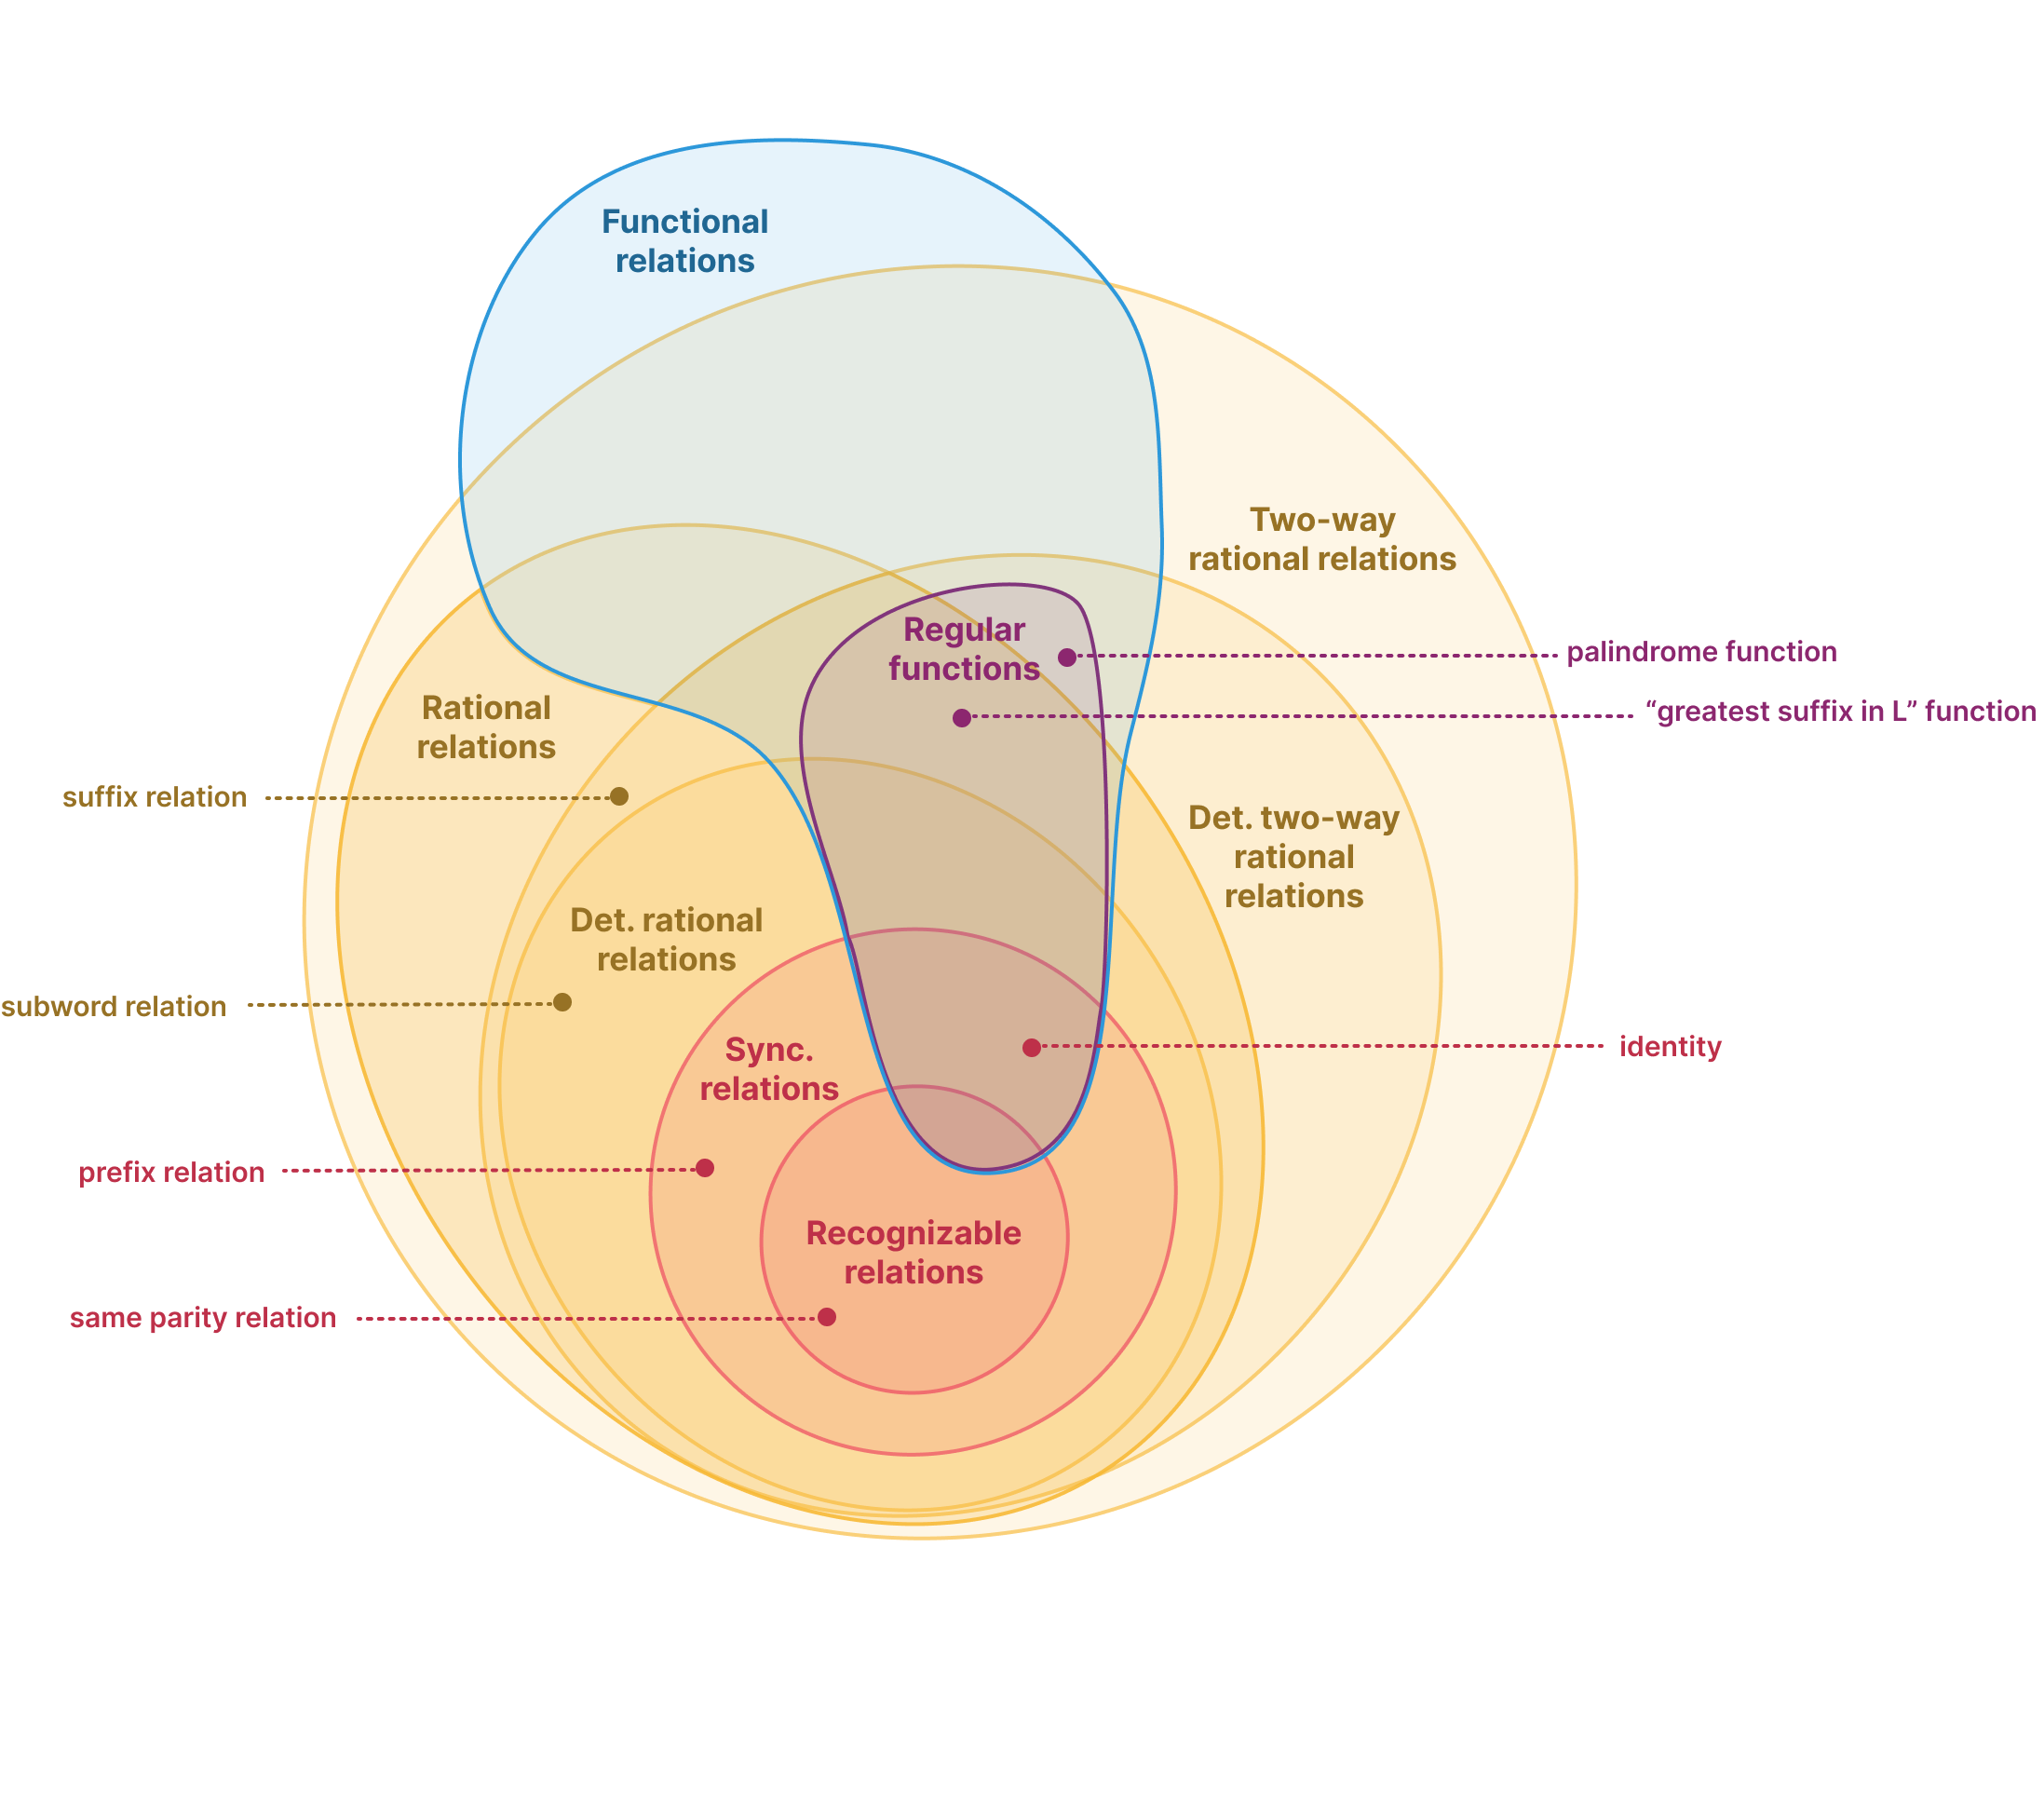
\includegraphics[width=\linewidth]{fig/landscape-rationality-relations.png}
	\caption{
		\AP\label{fig:landscape-rationality-relations}
		The ``landscape of rationality'' for binary relations.
		Dashed regions are empty.
	}
\end{figure}
Often, in the literature, when the terminology ``transduction'' is used,
these relations are thought as functions from $\Gamma^*$ to $\pset{\Sigma^*}$---sometimes
assuming that the input is a singleton, sometimes not---,
and in this case $\Gamma$ (resp. $\Sigma$) plays the role of an ``input alphabet''
(resp. ``output alphabet''). On the other hand, when the terminology ``relation'' is used,
we often take $\Gamma = \Sigma$. This makes little difference since we can often
see a relation $\+R \subseteq \Gamma^* \times \Sigma^*$ as a subset of
$(\Gamma\sqcup \Sigma)^* \times (\Gamma\sqcup \Sigma)^*$
while preserving the notion of ``rationality'' at hand.


\subsection{Recognizable Relations}

A relation $\+R \subseteq \Gamma^* \times \Sigma^*$ is \AP""recognizable@@rel""
if there exists a "finite monoid" $\?M$ together with a "monoid morphism"
\[
	f\colon \Gamma^* \times \Sigma^* \to \?M,
\]
as well as a subset $\Acc \subseteq M$ "st"
$\+R = f^{-1}[\Acc]$.
For instance the \AP""same parity relation""
\[
	\SameParity \defeq 
	\{
		\tup{u,v} \in \Gamma^* \times \Sigma^* \mid
		|u| = |v| \mod{2}
	\}
\]
is "recognizable". Indeed, letting $f\colon  \Gamma^* \times \Sigma^* \to \ZnZ{2}$,
then $\SameParity$ can be written as $f^{-1}[\{\bar 0\}]$.

These relations admit a remarkably simple characterization.\AP
\begin{proposition}[{""Mezei's theorem"", see "eg" \cite[Corollary~II.2.20, p.~254]{Sakarovitch2009Elements}}]
	\!\footnote{\cite[\S~2, ``Notes \& references'']{Sakarovitch2009Elements} mentions
	that this proposition is ``unanimously ascribed to G. Mezei (unpublished)''.}
	\label{prop:Mezei-theorem}
	A relation $\+R$ is "recognizable" "iff" there exists $n\in\N$,
	"regular languages" $\tup{K_i}_{i\in \lBrack 1,n\rBrack}$ over $\Gamma$
	and "regular languages" $\tup{L_i}_{i\in \lBrack 1,n\rBrack}$ over $\Sigma$
	"st"
	\[
		\+R = \bigcup_{i=1}^n K_i \times L_i.
	\]
\end{proposition}

For instance, $\SameParity =
(\Gamma\Gamma)^* \times (\Sigma\Sigma)^*
\cup \Gamma(\Gamma\Gamma)^* \times \Sigma(\Sigma\Sigma)^*$.
We now provide a slightly more general statement of "Mezei's theorem".

\begin{proposition}
	\label{prop:Mezei-theorem-generalization}
	Let $\B{V}$ be a "pseudovariety of finite monoids"
	and $\+V$ be the corresponding "pseudovariety of regular languages".
	A relation $\+R \subseteq \Gamma^* \times \Sigma^*$ is "recognizable@@rel"
	if, and only if, there exists $n \in \N$
	and $K_1,\hdots,K_n \in \+V_{\Gamma}$ and $L_1,\hdots,L_n \in \+V_{\Sigma}$
	"st" $\mathcal{R} = \bigcup_{i=1}^n K_i \times L_i$.
	% in which case we say that $\+R$ is \AP""$\+V$-recognizable"".
\end{proposition}

When $\B{V}$ is the "pseudovariety@@reglang" of all "regular languages",
we get back \Cref{prop:Mezei-theorem}.

\begin{proof}
	\proofcase{From monoids to products.}
	Assume that $\+R$ is "recognizable@@rel". 
	Then by definition
	\[
		\+R = \bigcup_{z \in \Acc} f^{-1}[z].
	\]
	Observe then that $f(u,v) = f(\tup{u,\varepsilon}\cdot\tup{\varepsilon,v})
	= f(u,\varepsilon)\cdot f(\varepsilon,v)$ for all $u,v \in \Gamma^* \times \Sigma^*$, and hence:
	\[
		\+R = \bigcup_{\substack{x,y \in M\\ \text{"st" } x\cdot y \in \Acc}}
		\underbrace{\{u \in \Gamma^* \mid f(u, \varepsilon) = x\}}_{\defeq \;K_x}
		\times \underbrace{\{v \in \Sigma^* \mid f(\varepsilon, v) = y\}}_{\defeq \;L_y}.
	\]
	Since $M$ is finite, the union is finite, and moreover, each $K_x$ and $L_y$ is
	recognized by $M$, and hence belong to $\+V$.

	\proofcase{From products to monoids.} If $\mathcal{R} = \bigcup_{i=1}^n K_i \times L_i$ 
		where all languages belong to $\+V$, then let $M_i,N_i \in \B{V}$
		be their "syntactic monoids", $g_i,h_i$ be their
		"syntactic morphism", and $\Acc_i,\Bcc_i$ be their accepting sets.
		Consider the monoid morphism
		\begin{center}
		\begin{tabular}{ccc}
			$\Gamma^* \times \Sigma^*$ & $\to$ & $\prod_{i}(M_i \times N_i)$ \\
			$\tup{u,v}$ & $\mapsto$ & $\tup{g_i(u), h_i(v)}_{i}$.
		\end{tabular}
		\end{center}
		Then $\+R$ is the preimage by this morphism of
		\[
			\bigcup_{i=1}^n \bigl(
			\cdots \times (M_{i-1}\times N_{i-1}) \times
			(\Acc_i \times \Bcc_i) \times (M_{i+1}\times N_{i+1}) \times \cdots \bigr).
		\]
		The conclusion follows from the fact that $\B{V}$ is closed under finite products.
\end{proof}

\Cref{prop:Mezei-theorem} proves that "recognizable relations" are not very expressive.
\begin{corollary}
	\!\footnote{Of course, this property is far from being sufficient
	at characterizing "reflexive relations": note that the proof
	does not even use the "regularity@@lang" of the languages at hand...}%
	\footnote{Of course, another way of proving this result would be
	to apply "Raysey's infinite theorem" to $f\colon \Sigma^* \times \Sigma^* \to \?M$.
	Again, we do not use the fact that $f$ is a "monoid morphism", but simply
	that it is a finite-domain function.}
	\AP\label{coro:infinite-clique-recognizable}
	Let $\+R \subseteq \Sigma^* \times \Sigma^*$ be a "reflexive relation".
	Then $\+R$ contains an infinite clique, "ie"
	there exists an infinite language $L \subseteq \Sigma^*$ "st"
	$\tup{u,v} \in \+R$ for all $u,v \in L$.
\end{corollary}
\begin{proof}
	Indeed, by \Cref{prop:Mezei-theorem}, write $\+R$ as $\bigcup_{i=1}^n K_i \times L_i$.
	Given a word $u \in \Sigma^*$, define $f(u) \in \?2^{2n}$ where
	the $2i$-th (resp. $(2i+1)$-th) bit of $f(u)$ indicates if $u \in K_i$ (resp. $u \in L_i$)
	for all $i$.
	By pigeon-hole principle, there exists a bit-sequence in $\?2^{2n}$ whose preimage
	$L$ by $f$ is infinite. Then pick $u,v \in L$. Since $\+R$ is reflexive, then
	$\tup{u,u} \in \+R$ and so, since $f(u) = f(v)$, we
	have $u \in K_i$ "iff" $v \in K_i$ and
	$u \in L_i$ "iff" $v \in L_i$ for all $i$, and so $\tup{u,v} \in \+R$.
\end{proof}

In particular, this corollary implies that neither the \AP""prefix relation""
$\intro*{\prefixRel} \defeq \{
	\tup{u,v} \in \Sigma^*\times\Sigma^* \mid
	\text{$u$ is a prefix of $v$}
\}$, the \AP""suffix relation""
$\intro*{\prefixRel} \defeq \{
	\tup{u,v} \in \Sigma^*\times\Sigma^* \mid
	\text{$u$ is a prefix of $v$}
\}$, nor the equality relation are "recognizable@@rel".
A similar proof can show that the ""equal-length relation""
$\intro*\equalLength \defeq \{
	\tup{u,v} \in \Gamma^*\times\Sigma^* \mid
	|u| = |v|
\}$.%
\footnote{Note however that \Cref{infinite-clique-recognizable} does not apply since
we assumed there that the input and output alphabets are equal.}


\subsection{Automatic Relations}



\subsection{Todo}

\begin{itemize}
	\item todo:add polyregular functions.
	\item todo: rename ``synchronous relations'' to ``automatic relations''
	\item todo:the intersection of
	functional relations and two-way rational relations
	collapses to regular functions by
	\cite[Theorem 22, p.~243]{EH2001transduction}.
	\item cite Gaëtan's thesis (chapter 1 for finite words, chapter 8 for infinite words)
	\item mention pebble, marble and whatnot.
\end{itemize}


\begin{itemize}
	\itemAP padding symbol $\intro*\pad$
	\itemAP convolution of words $\intro*\convol$
	\itemAP convolution of a relation $\intro*\convolRel{\+R}$
	\itemAP ""automatic relation"" and $\intro*\AUT$
\end{itemize}